\chapter{Modelling the deformation of hollow objects in real-time}
\label{chap7}
\begin{shortAbstract}
The human body is composed of various deformable anatomical structures and finding appropriate soft-tissue models for all these type of structures is challenging. In the previous two chapters, we described an efficient non-linear FEM formulation for simulating the deformation of solid organs (like brain, liver, prostate etc.). But there is also a need to simulate the deformation of hollow organs, whose volume is negligible compared to their surface area, such as colon, blood vessels, stomach etc. The solid models previously mentioned are not appropriate and specific approaches are required for these thin anatomical structures. In this chapter, we will review diverse techniques applied for the simulation of thin objects. These different approaches may be grouped into three main categories: (1) mass-spring models, (2) approaches which derive a bending energy from geometrical considerations and (3) methods based on the equations of continuum mechanics. Although very few models have been proposed for simulating the deformation of thin anatomical structures in the field of medical simulation, we will try to emphasize medical applications whenever possible. 
\end{shortAbstract}


\section{Introduction: the problematic}
The human body is composed of various deformable anatomical structures. A key challenge of soft-tissue modelling is the variousness of the mechanical behaviours. The shape and the internal structure may be very different from one organ to another. If you take the liver for instance, it is a solid organ composed of four lobes, each one made up of units called lobules. Each lobule consists of a central vein surrounded by liver cells and constitutes the end of a dense network of blood vessels. This particular internal structure has a strong influence on the mechanical properties of the liver. In contrast, the colon is a long and hollow organ. It consists of four sections which all have different shapes and material properties. Consequently, it seems unrealistic to use a unique model for all tissues. Yet, most of previous works focus on volumetric models that are able to capture the behaviour of solid organs. In fact in the field of medical simulation, very few models have been proposed for simulating, in real-time, the deformation of thin anatomical structures whose volume is negligible compared to their surface area. Examples include hollow structures, such as the wall of blood vessels, or membranes, such as the Glisson's capsule surrounding the liver. It is also of particular interest to us for modelling the colon in our colonoscopy simulator and for simulating the deployment of the implant in cataract surgery. 

The first idea that may come to mind for modelling thin structures is to apply the same methods than with solid objects. For instance, \cite{Holzapfel02} proposed a very complex 3-layer model of an aterial wall for simulating an angioplasty procedure. Their model is non-linear and anisotropic along fibers placed according to histology. They also model diseased part of the vessel through a hardening parameter which adds plasticity. However, they discretised their geometric model with eight-node brick elements. Another example is given by \cite{Aloisio04} who assume that the blood flow in the vessels may be considered as incompressible and the artery consequently becomes a solid body and can be modelled as a solid deformable object. \TODO{why is this not appropriate? High-order elements could do the trick of following the curvature...} Hence, specific models for thin objects were developed. 

Indeed, numerous models are available in the literature to describe physics of thin objects, from fairly simple and naive approaches to more complex and thorough representations. Continuum mechanics provides many formulations able to accurately describe stresses occurring within thin objects. Most of them fall into one of the following two categories: plate theory or shell theory. Those theories have been a subject of interest in the mechanical community for decades. The difference between these two kinds of structures is very well explained by \cite{Liu03} and can be summarised by the fact that plate bending elements can only carry transversal loads while shells can undergo more complex deformations. 
For instance, if we consider the horizontal board of a bookshelf, that board can be approximated as a plate structure and the transversal loads are the weight of the books. A typical deformation of the board is illustrated in \fig{chap7:fig-boards} (a). Conversely, a shell structure can carry loads in all directions, and therefore can undergo bending, twisting and membrane (that is, in-plane) deformation (see \fig{chap7:fig-boards} (b)). 
%
\begin{figure}[ht]
\centering 
\subfloat[Plate theory]{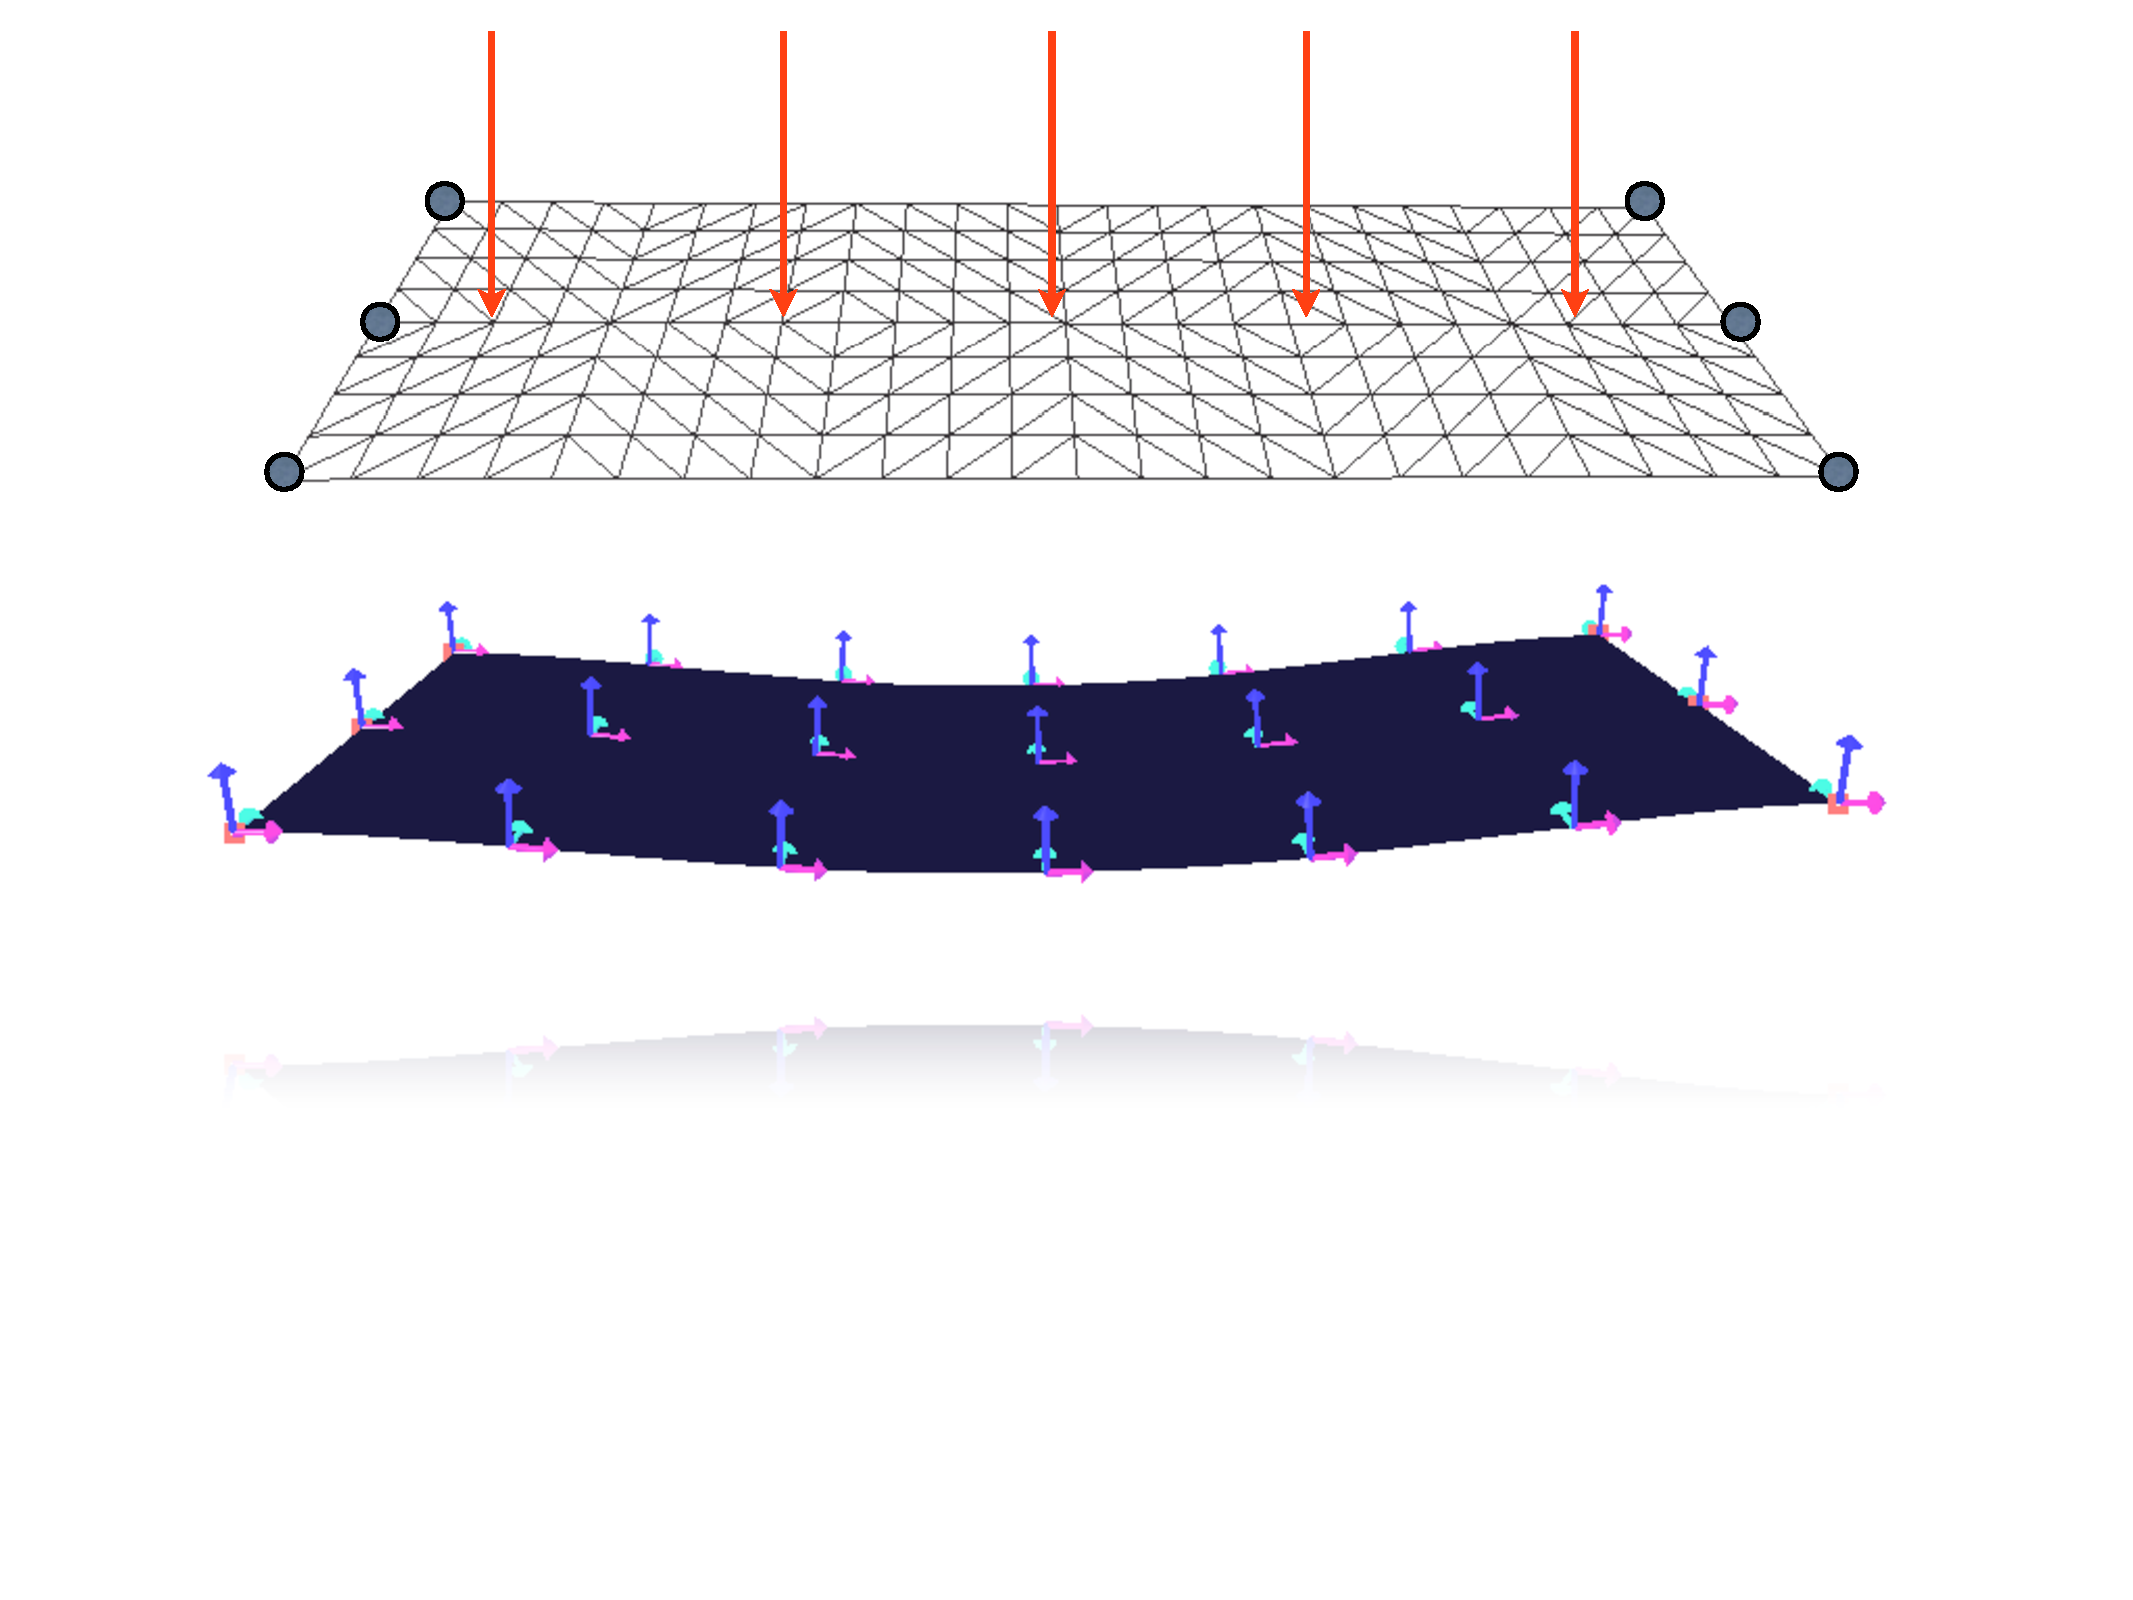
\includegraphics[width=6.5cm]{chapter7/board_bending.pdf}}
\hfill 
\subfloat[Shell theory]{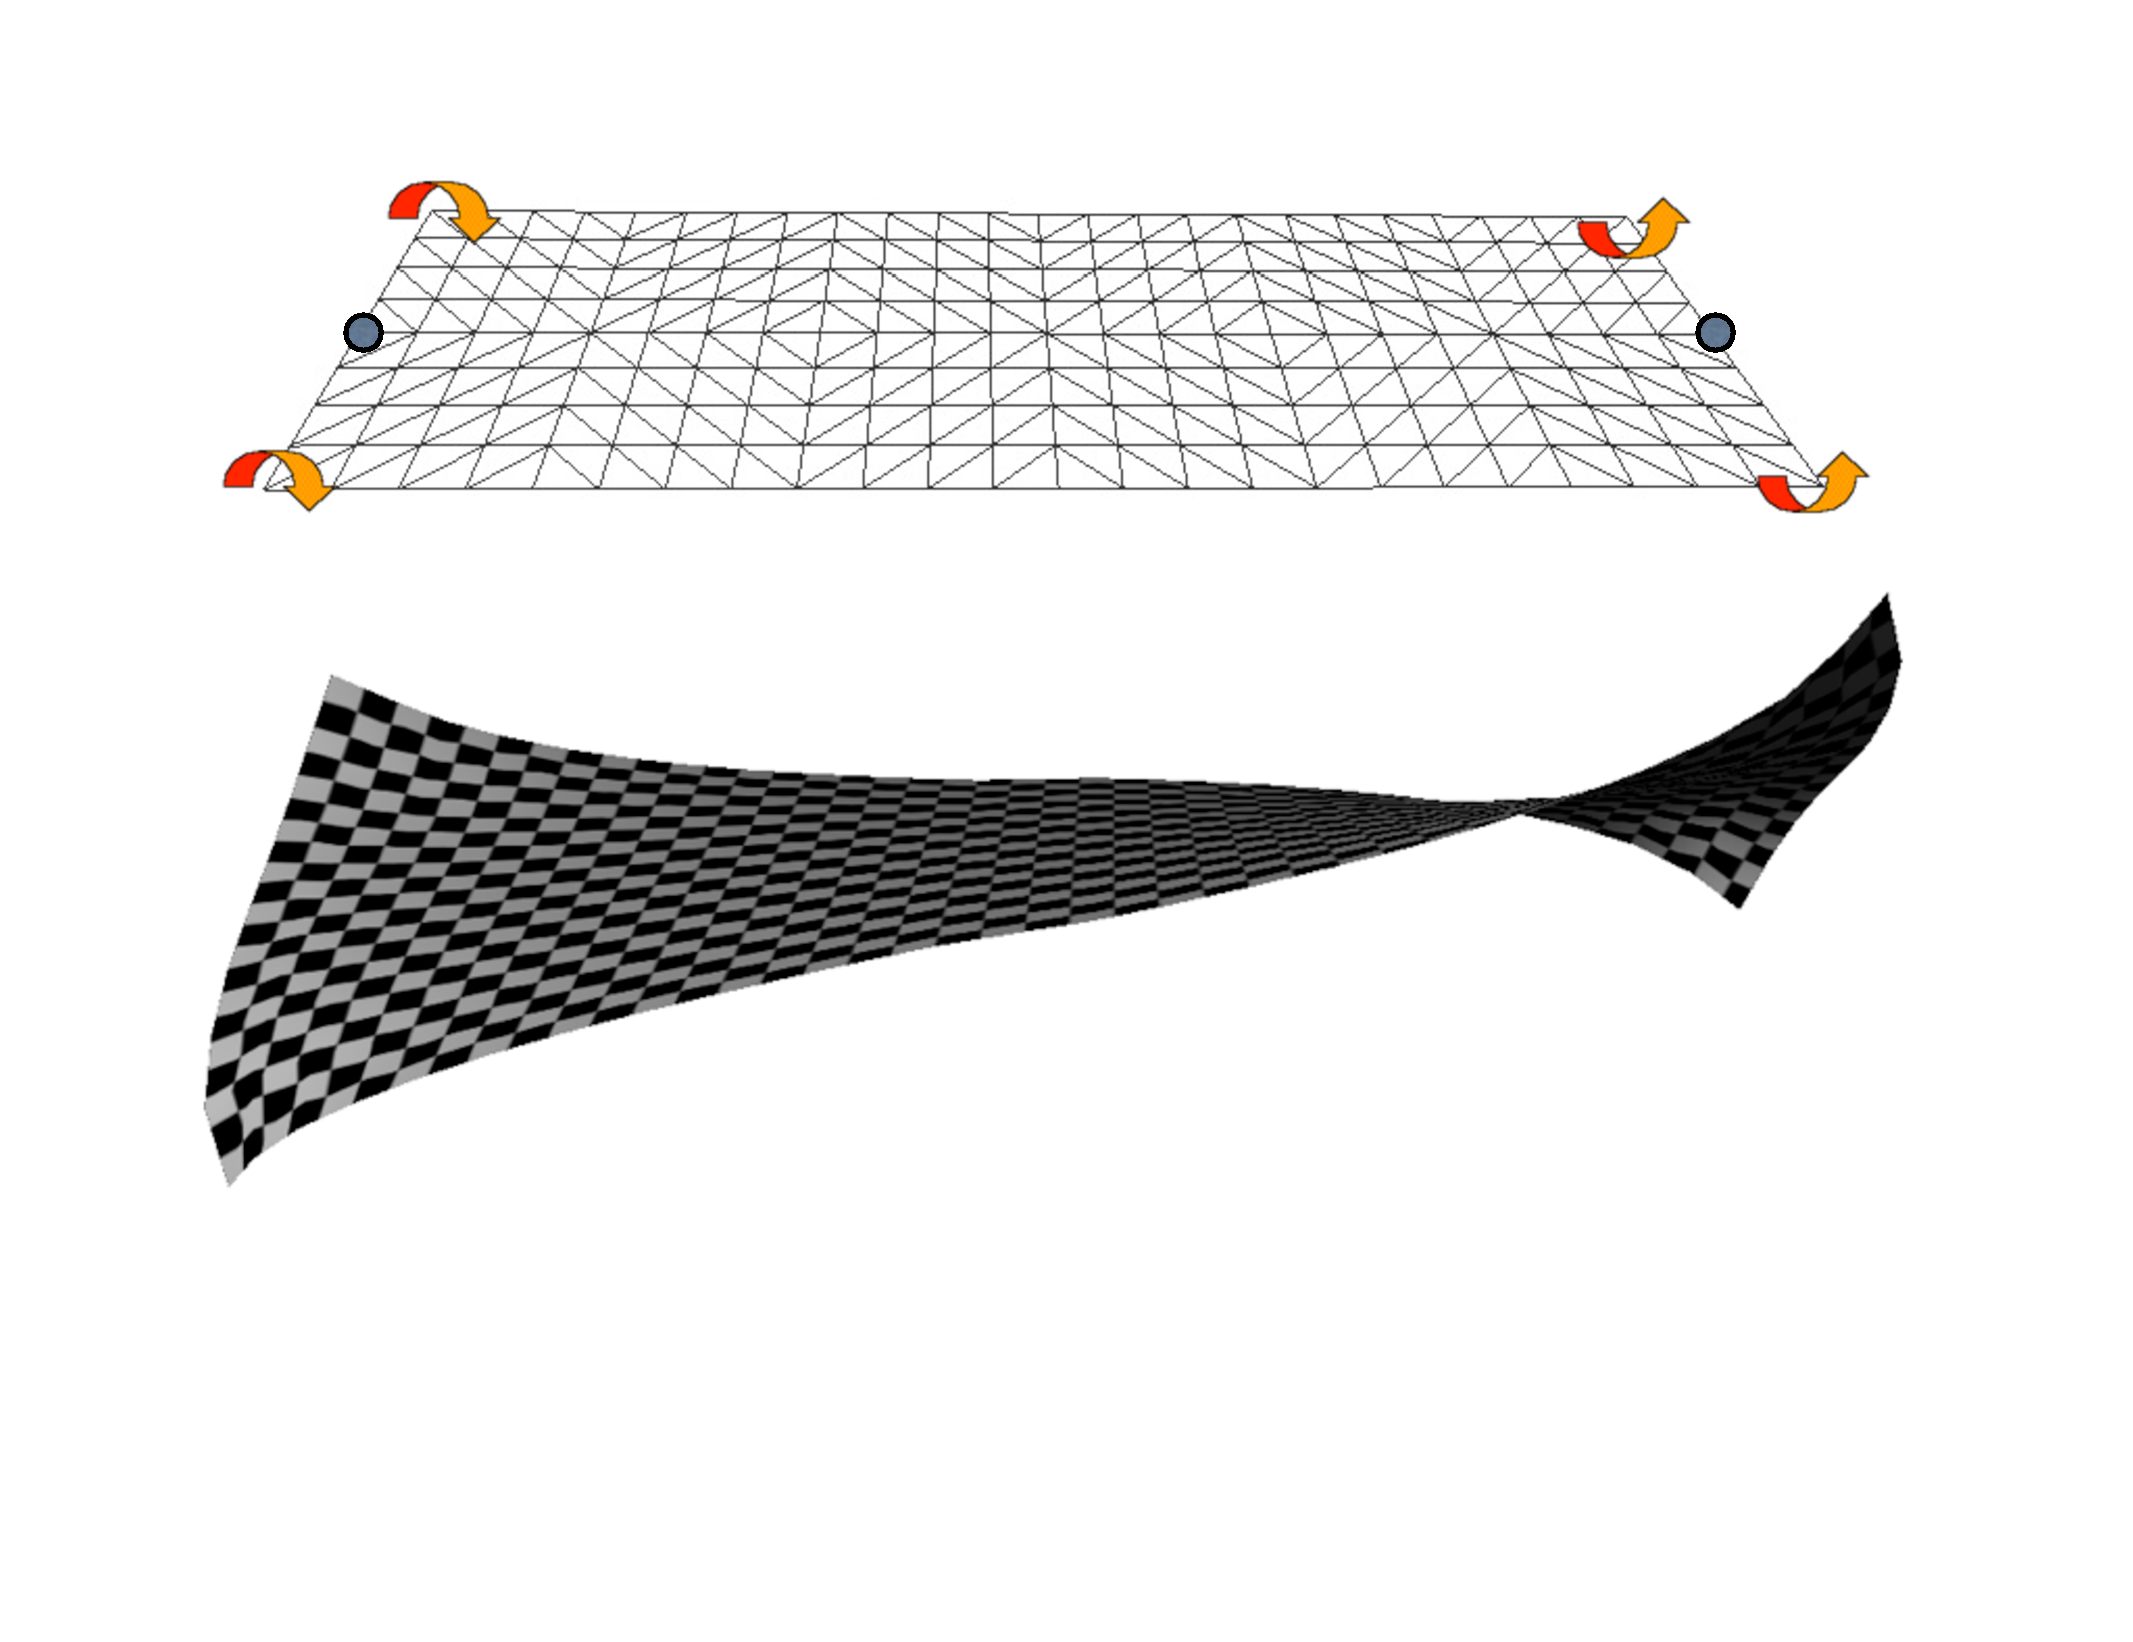
\includegraphics[width=6.5cm]{chapter7/board_twist.pdf}}
\caption[Illustration of the key difference between plate and shell theory]{Illustration of a key difference between various models of thin objects. While thin plate theory allows to describe bending (a), it cannot represent more complex deformations such as twist (b) which is captured by shell theory.}
\label{chap7:fig-boards}
\end{figure}


Development of a satisfactory physical model that runs in real-time but produces visually convincing animation of thin objects has been a challenge in Computer Graphics, particularly in the area of cloth modelling. Rather than resorting to shell theory which involves the most complex formulations in continuum mechanics, most of works have relied on discrete formulations. We will first discuss early approaches based on mass-spring models. Then we will present techniques relying on the derivation of a bending energy from geometric considerations. At last, we will introduce approaches based on shell theory using the more computationaly demanding finite element method.

%	\subsection{Colonoscopy simulator project: needs for colon}
%	\subsection{Cataract surgery, stenosis: other needs for implants/blood vessels}
		
\section{Mass-spring models}

Early approaches to thin objects modelling only considered in-plane deformation, and often relied on mass-spring models. This technique was already presented in section \ref{chap4:massSprings} so we only present their use for modelling thin structures. \cite{Provot95} improved a mass-spring model to take into account the non-elastic properties of woven fabrics. Because of the high stiffness of textiles, mass-spring models are particulary unstable when used to simulate cloth. The author proposed a new method inspired from dynamic inverse procedure. Under certain conditions and because of the linear law employed in a mass-spring system, the fabrics may become super-elastic. \citeauthor{Provot95} suggested to set a threshold on the deformation rate to correct this super-elasticity (see \fig{chap7:fig-sheet}). 
%
\begin{figure}[ht]
\centering 
\subfloat[Initial position]{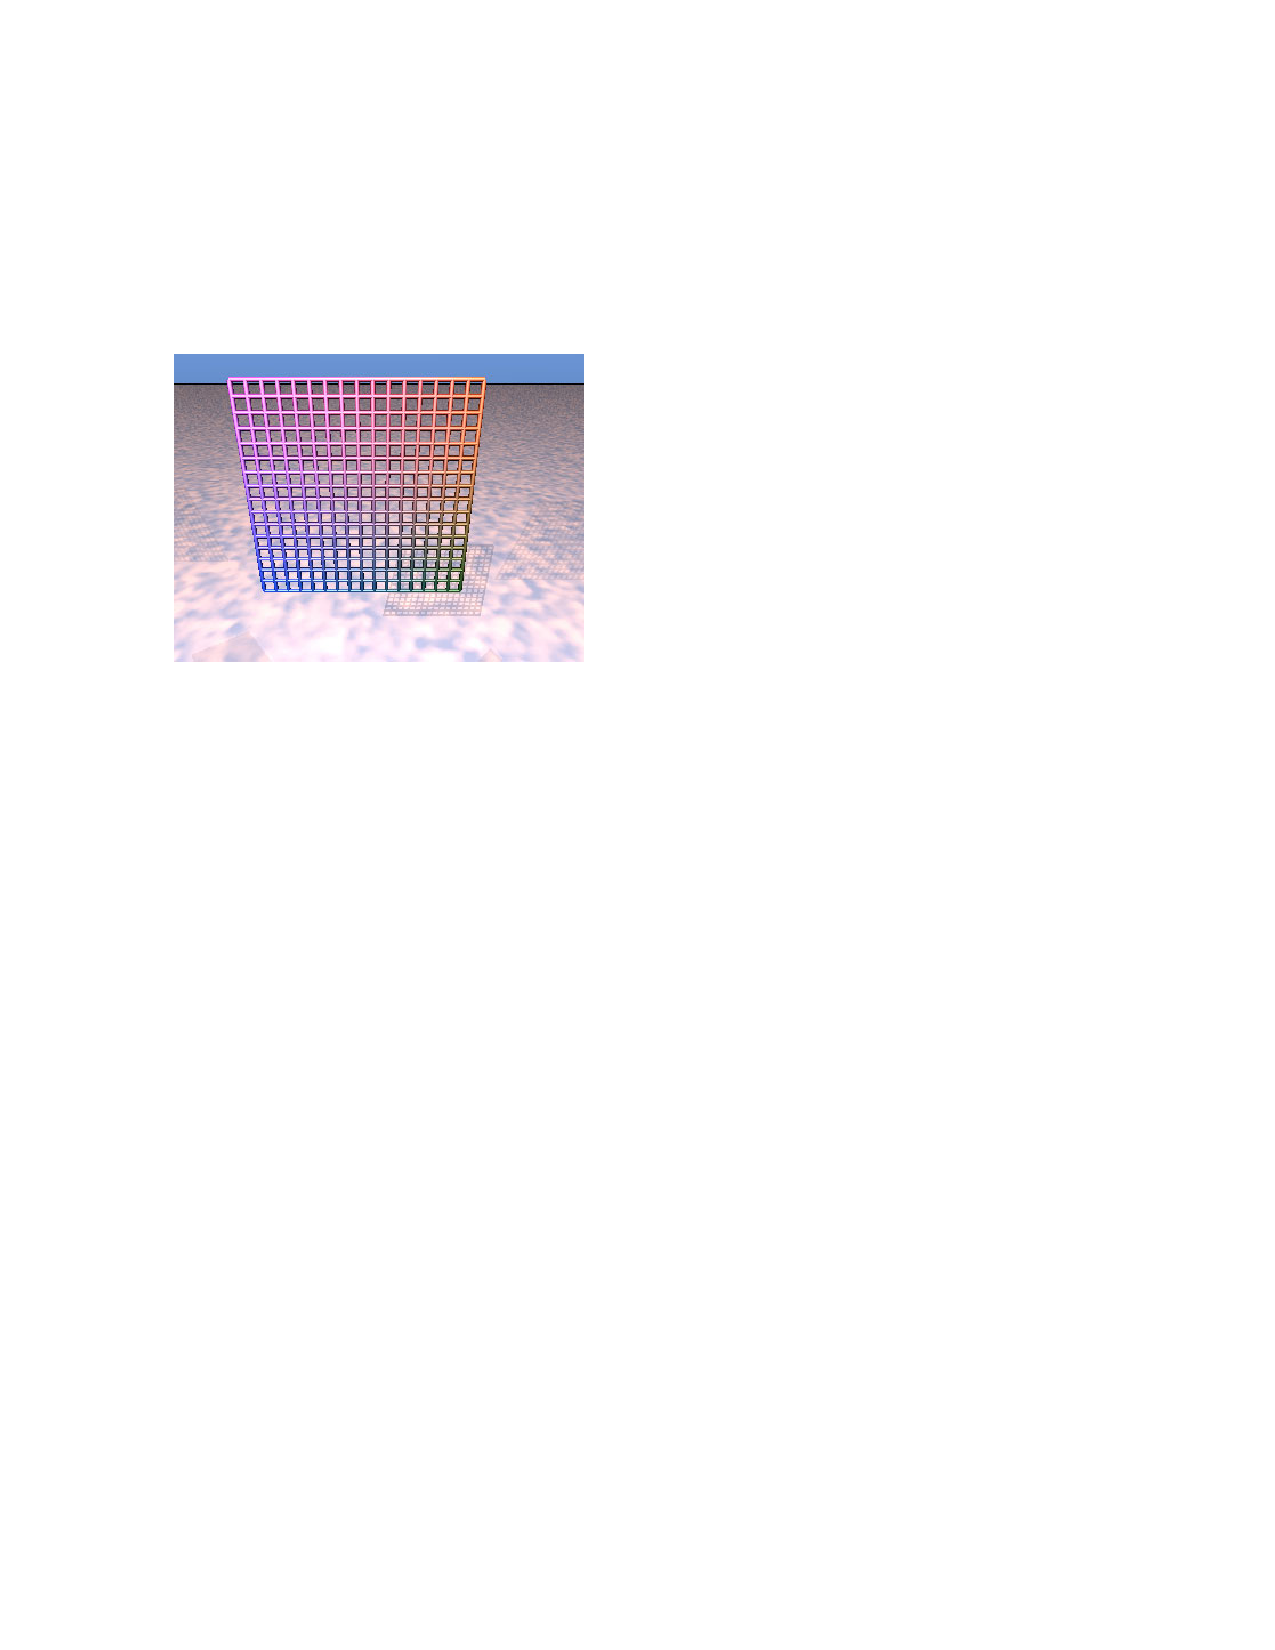
\includegraphics[width=4.5cm]{chapter7/sheet1.pdf}}
\hfill 
\subfloat[Uncorrected]{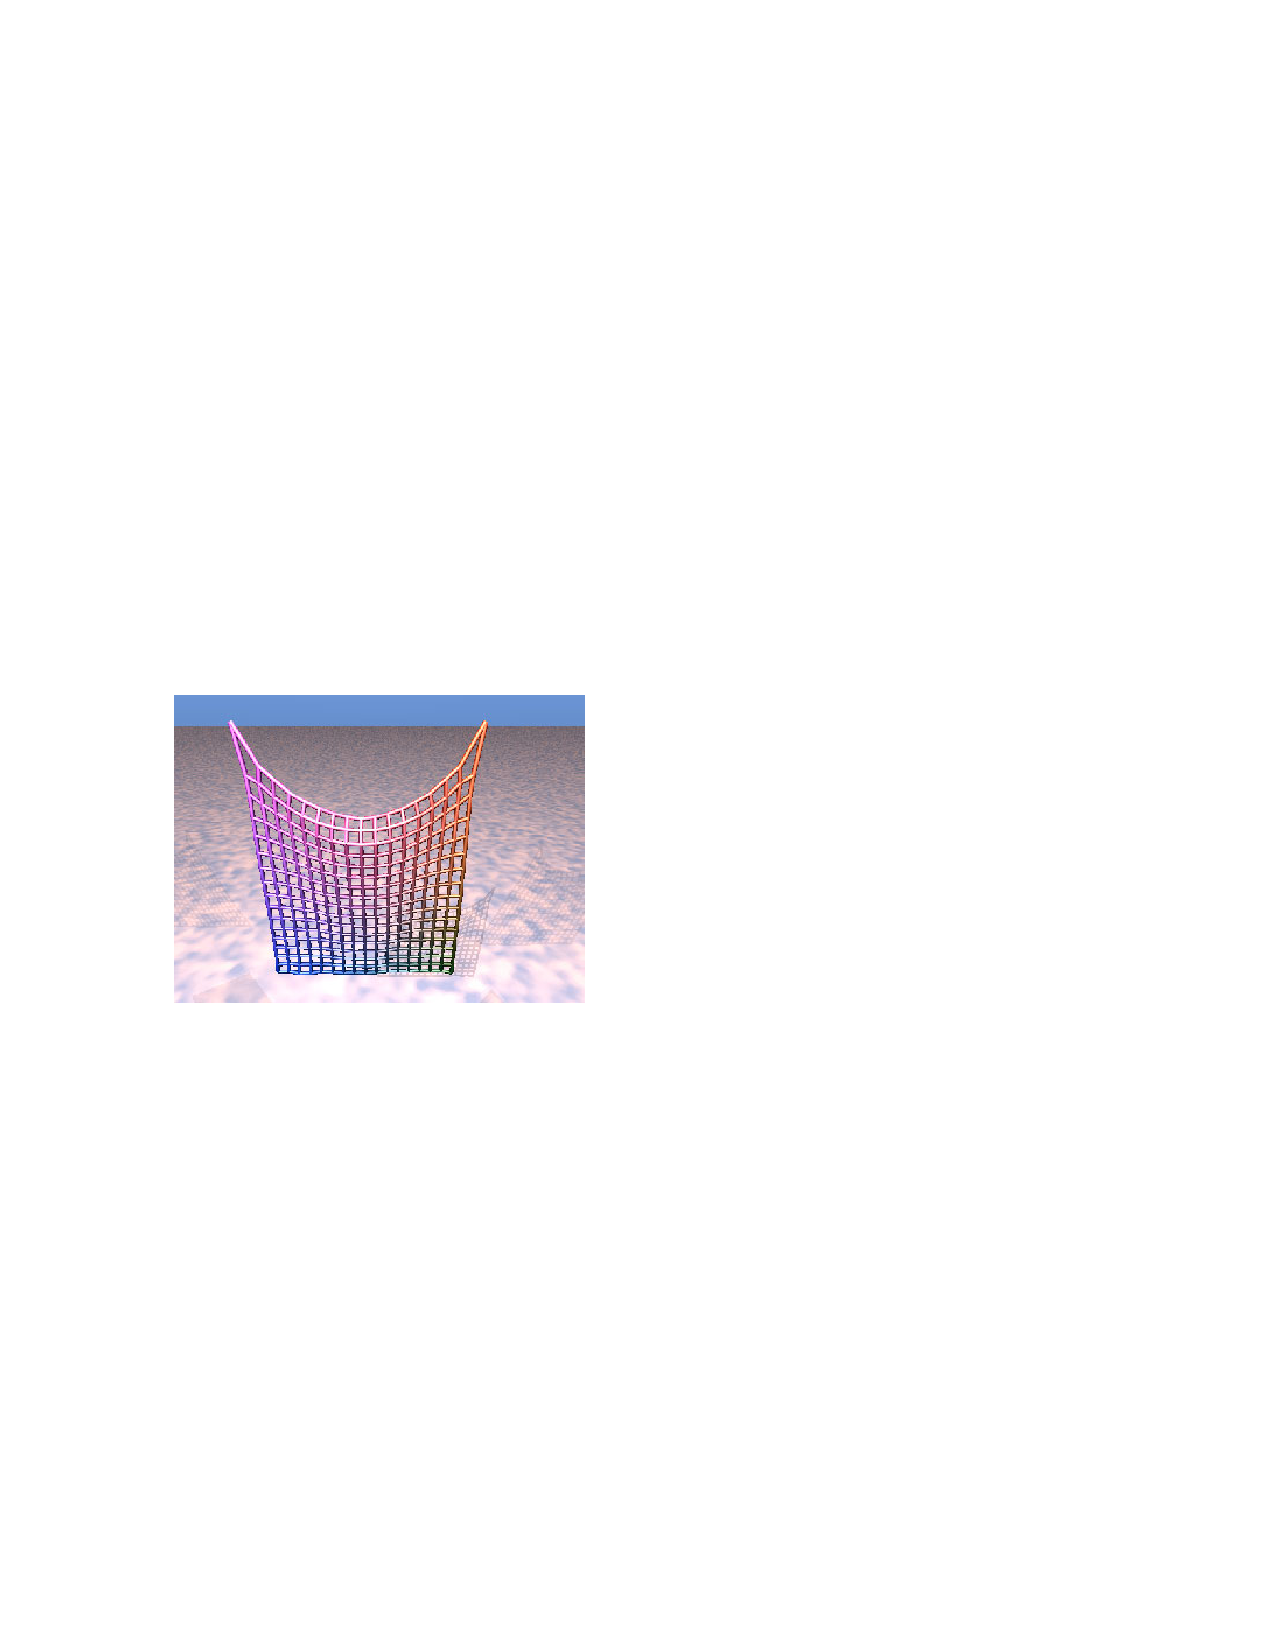
\includegraphics[width=4.5cm]{chapter7/sheet2.pdf}}
\hfill 
\subfloat[Corrected]{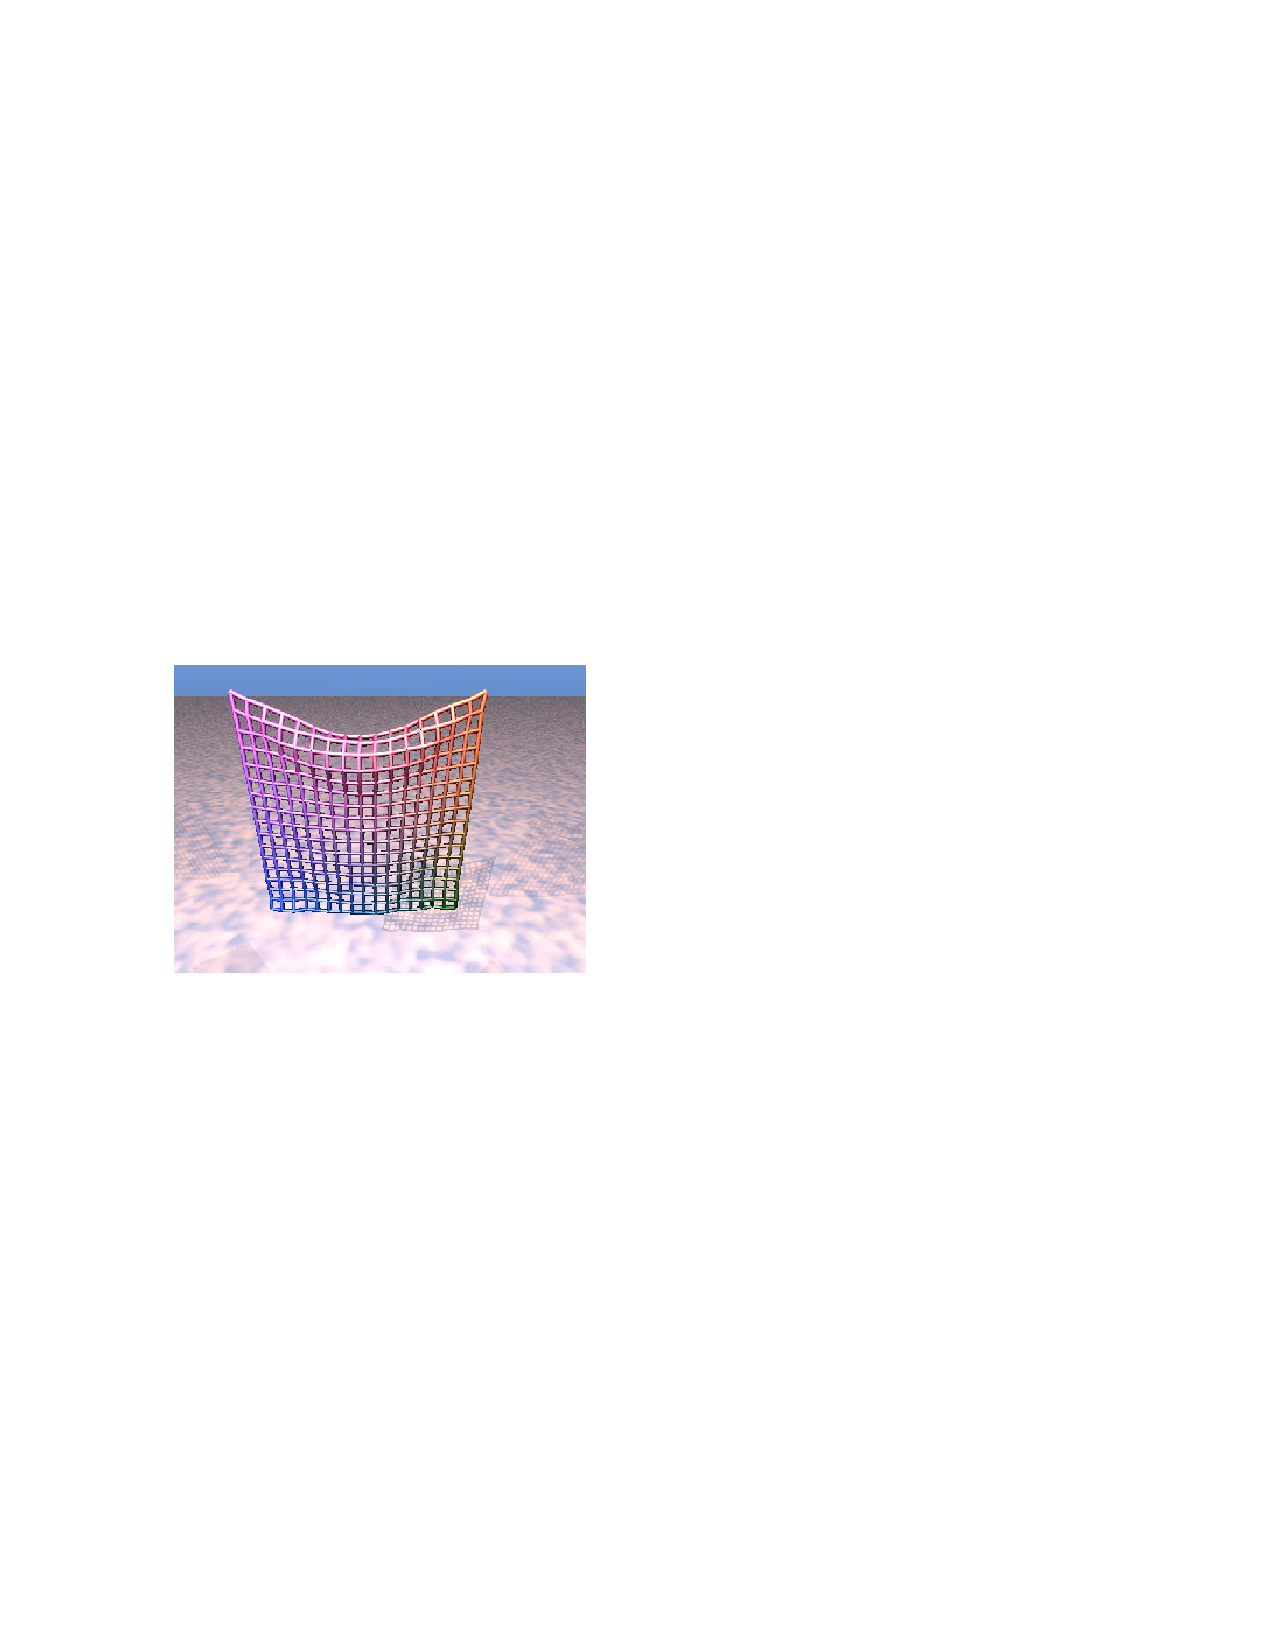
\includegraphics[width=4.5cm]{chapter7/sheet3.pdf}}
\caption{Deformation of a sheet hanging by two adjacent corners. Images courtesy of \cite{Provot95}.}
\label{chap7:fig-sheet}
\end{figure}

To improve the computational efficiency, \cite{Hutchinson96} presented a mechanism for adaptively refining the network of mass-springs to concentrate efforts only where it is needed. When potential inaccuracies are detected, the object is locally refined in the affected region, and the simulation may carry on. \cite{Oshita01} used a sparse triangular mesh and an interpolation to generate a dense mesh. 

A limitation of mass-spring models that we often hear is the difficulty to derive spring stiffness from elastic properties (Young's modulus and Poisson's ratio). With this drawback in mind, \cite{Volino97} improved a mass-spring system by allowing the modelisation of Young's modulus and Poisson's ratio (see \fig{chap7:fig-fabricSquares}). They also added a correction technique relying on the control of damping and velocities to ensure the stability of their model. 
%
\begin{figure}[ht]
\begin{center}
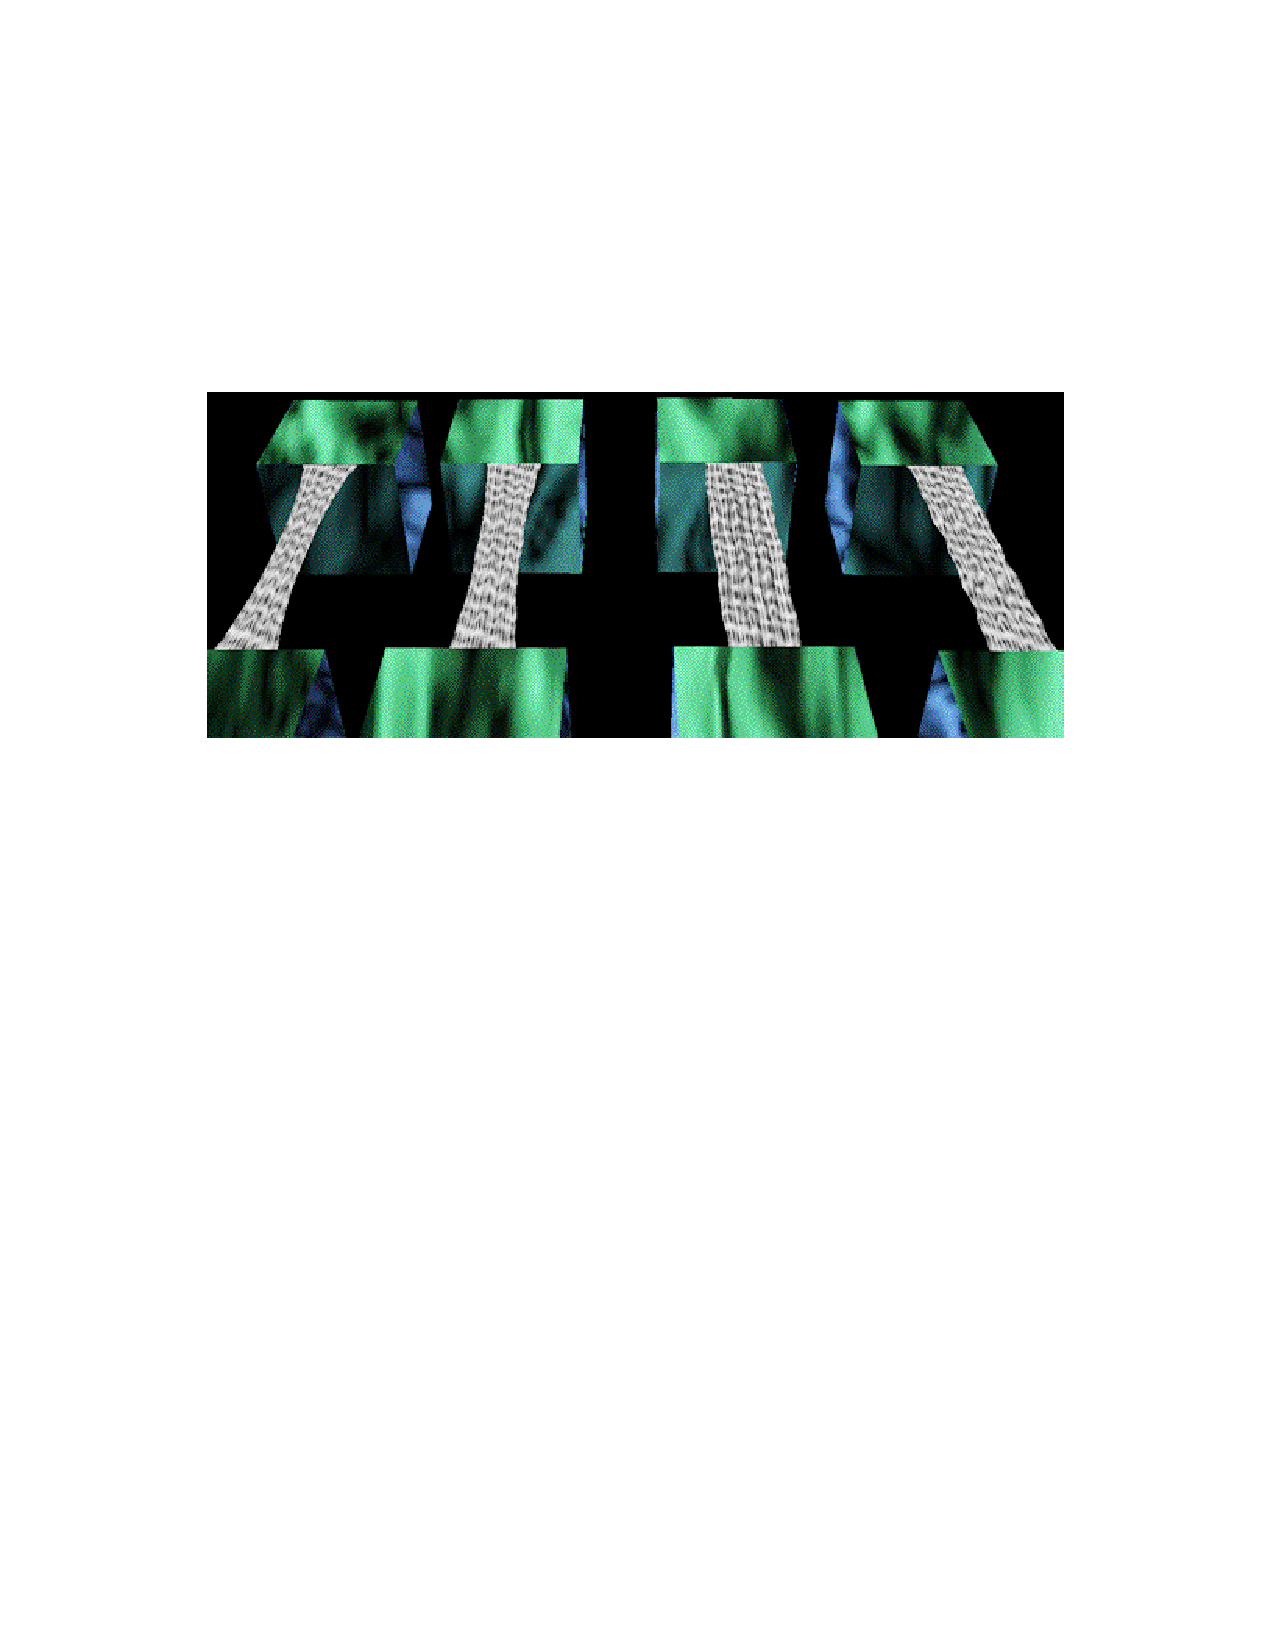
\includegraphics[width=12cm]{chapter7/fabricSquares.pdf}
\caption[A $400\,$\% stretched fabric square]{A $400\,$\% stretched fabric square with various Poisson's ratio. Image courtesy of \cite{Volino97}.}
\label{chap7:fig-fabricSquares}
\end{center}
\end{figure}

Other works have considered adding bending through angular springs. For instance, \cite{Taskiran05} have chosen to use a linear representation of angular springs to supply bending and torsion effects in hair modelling, which allowed them to simulate curly hair with good realism. All the forces related to springs were implemented: gravity, repulsions from collision, absorption, friction, etc. They could simulate up to a few hundreds of hair stripes in real-time. \cite{Wang07} successfully used a network of linear and angular springs to describe bending and twisting of catheters and guidewires in an interventional radiology simulator. 

More recently and in the field of medical simulation, \cite{Hammer08} employed a mass-spring model to simulate the mitral valve closure for surgical planning. In their model, triangle sides are treated as linear springs and sides shared by two triangles are treated as bending springs. 

	
\section{Techniques relying on the derivation of a bending energy}

Another kind of approach is to geometrically derive a bending energy. Theses approaches are more computationally demanding than mass-spring models but allows for higher flexibility and accuracy. For instance, \cite{Baraff98} derived stretch, bending and shear energies geometrically. They also used an adaptative time stepping based on detection of large stretches. Using an implicit integration allows the authors to use large time steps and substantially increase the stiffness with a limited impact on performance. 

Among the geometry-based models, there is the noticeable work of \cite{Grinspun03} who introduced a discrete shell model. They designed a simple shell model for triangle meshes by geometrically deriving membrane and bending energies. They applied geometric operators over piecewise-linear surfaces to define a discrete constitutive model, which results in simpler expressions than tensorial derivations from shell theory. They applied their method to simulate the deformation of common objects like beams, sheets of paper or hats (see \fig{chap7:fig-hat}). 
%
\begin{figure}[ht]
\begin{center}
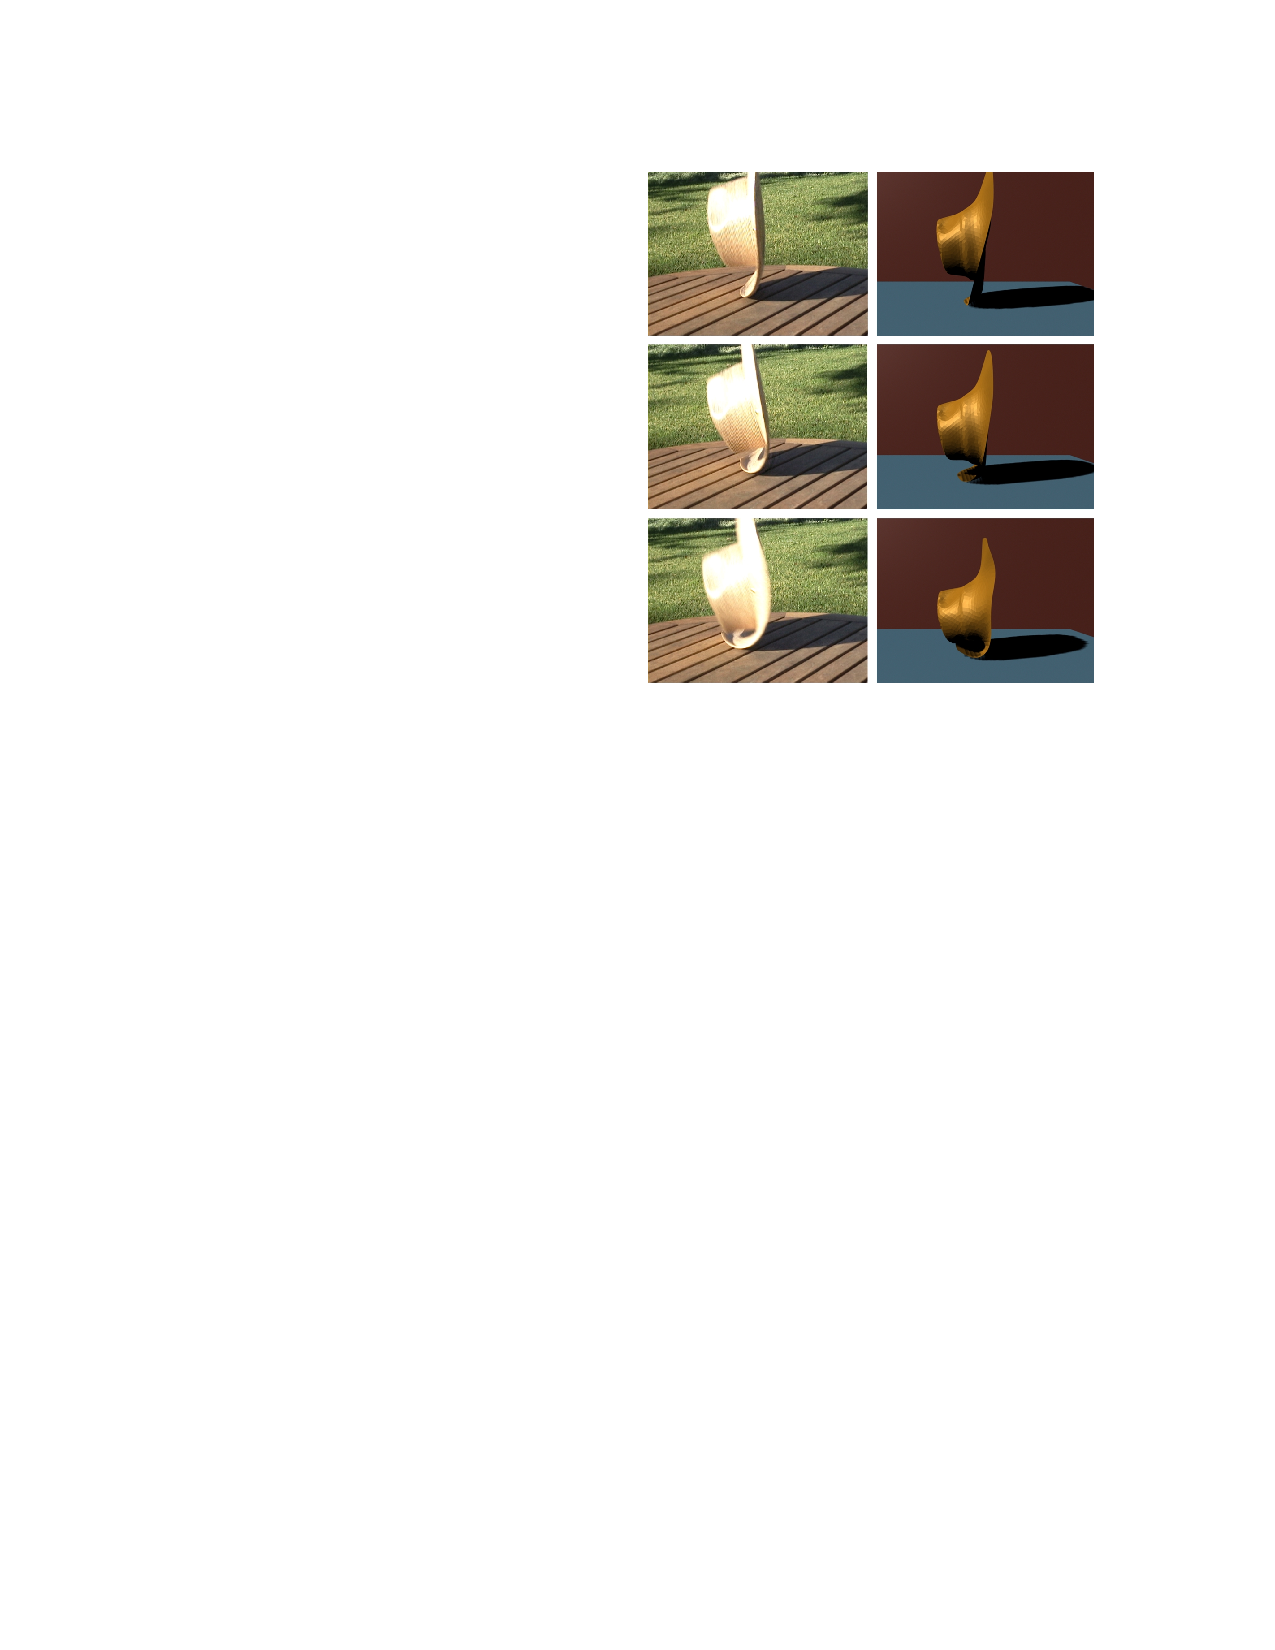
\includegraphics[width=9cm]{chapter7/hat.pdf}
\caption[Comparison between real footage and simulation of a hat dropped on a table]{Comparison between real footage and simulation of a hat dropped on a table. Image courtesy of \cite{Grinspun03}.}
\label{chap7:fig-hat}
\end{center}
\end{figure}

Among the different models introduced recently we can also mention the work of \cite{Choi07} and \cite{Bridson03}. \citeauthor{Choi07}  proposed a real-time simulation technique for thin shells undergoing large deformations. The authors adopt the energy functions from the discrete shells proposed by \cite{Grinspun03}. For real-time integration of the governing equation, they adapted a modal analysis technique, called modal warping. The resulting simulations run in real-time even for large meshes, and the model can handle large bending and/or twisting deformations with acceptable realism. \citeauthor{Bridson03} followed the same energy approach to derive their bending model but improved the resolution of the equations by suggesting a novel mixed implicit/explicit integration scheme. In particular, the explicit update for positions allows the authors to modify velocities to enforce constraints and allows a strain limiting procedure which they used to create folds and wrinkles in their cloth simulation. They also presented a post-processing method for treating cloth-character collisions that preserves folds and wrinkles. \cite{Pabst08} later improved the bending modelling used by \citeauthor{Bridson03} to allow the integration of measured material data. 

\cite{Volino06} suggested an alternative somewhere between mass-spring and geometrically derived approaches. They compute a bending vector that represents the bending of the surface through  a simple linear combination of particule positions and they distribute this vector as particule forces according to the bending stiffness. The authors claimed much better accuracy than mass-spring models (particulary when dealing with low curvature and high bending stiffness) with similar computation time (see \fig{chap7:fig-dress} for an illustration). 
%
\begin{figure}[ht]
\begin{center}
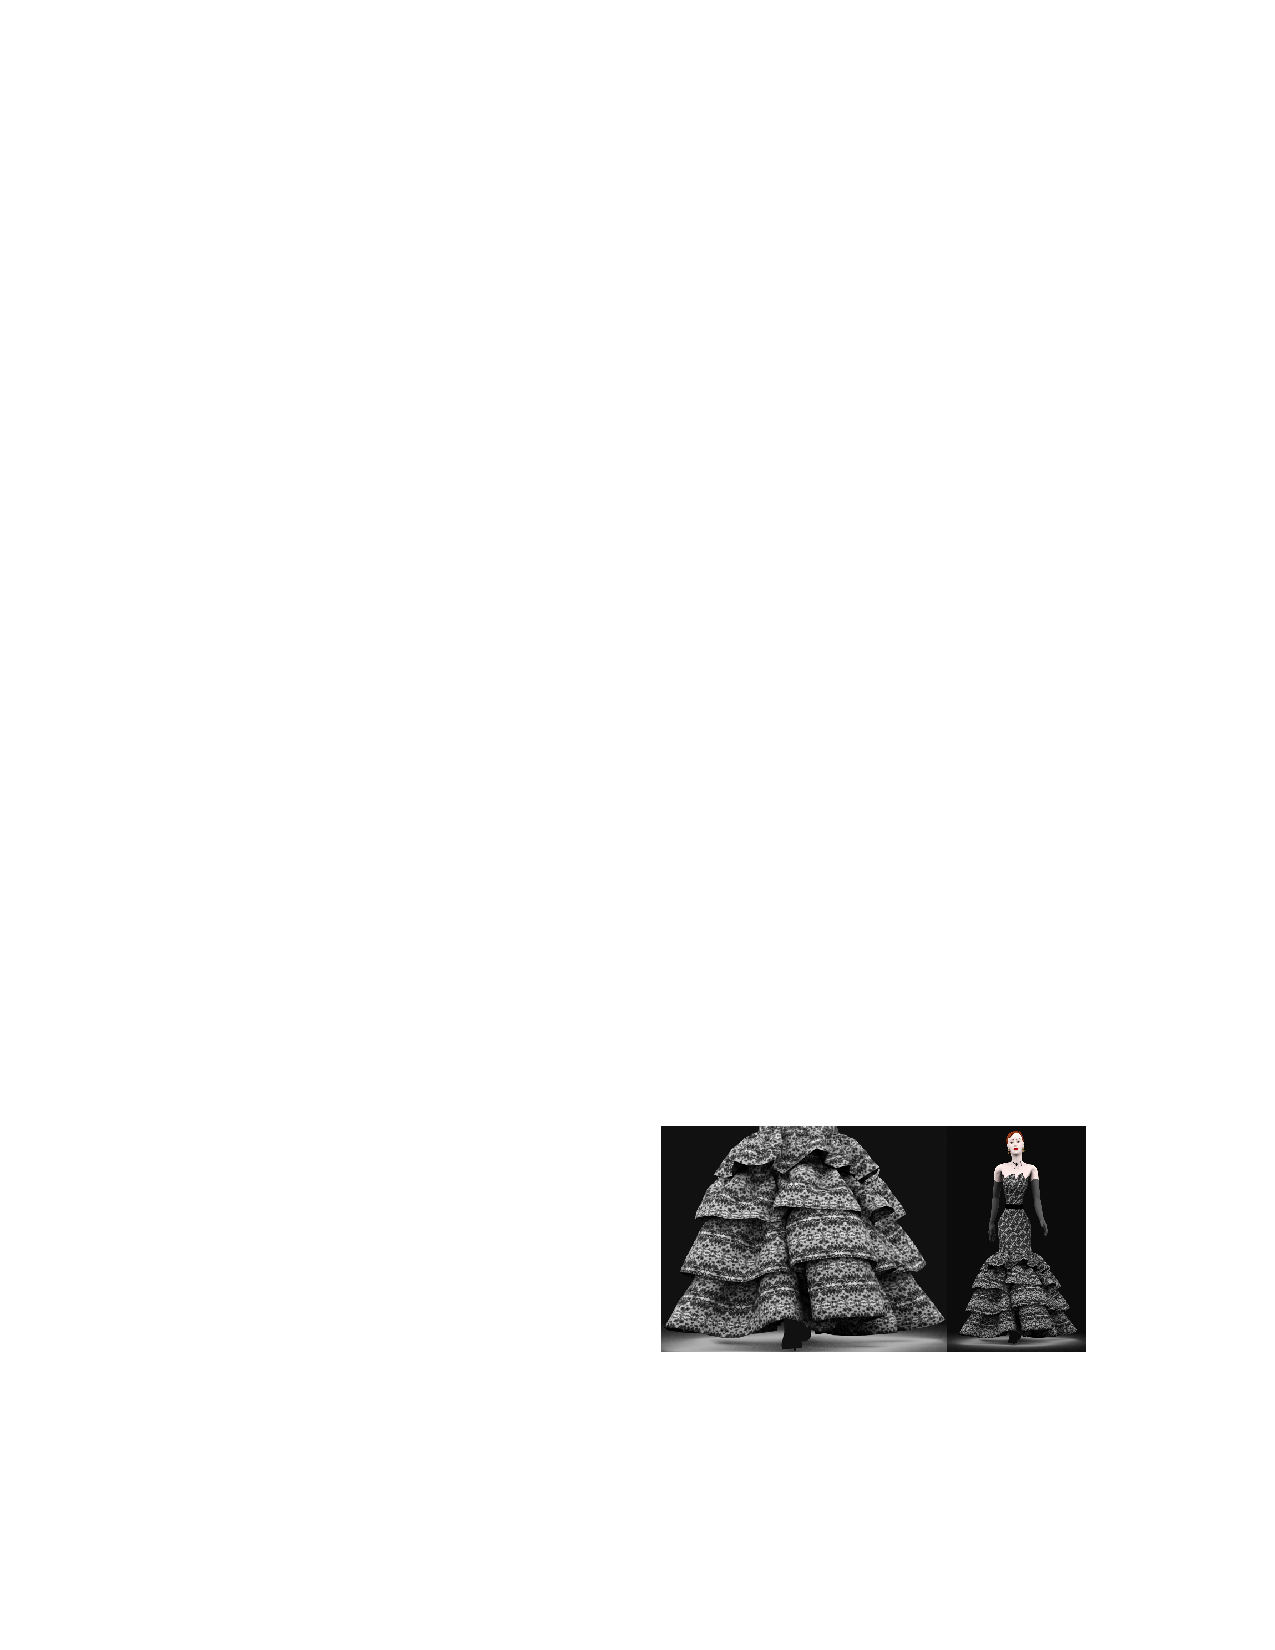
\includegraphics[width=10cm]{chapter7/dress.pdf}
\caption[Simulation of complete garments that have large bending stiffness]{The model of \citeauthor{Volino06} allows the simulation of complete garments with material that may have fairly large bending stiffness. Image courtesy of \cite{Volino06}.}
\label{chap7:fig-dress}
\end{center}
\end{figure}

A method to use thin shell dynamics with point sampled surfaces for efficient animation was recently proposed by \cite{Wicke05} where the curvature of the shell is measured through the use of fibers. The fibers are used to approximate the differential surface operators. Their method supports both elastic and plastic deformations as well as fracturing and tearing of the material. 
		

\section{Techniques based on continuum mechanics}

Following a similar train of thoughts than with solid objects, methods based on continuum mechanics provide the most accurate solutions but are computationally very demanding. The mathematical framework of plate and shell theories is also fairly complex and deriving finite element methods from these theories is challenging. Their implementation is also far from being straightforward. Nevertheless, we will now review a few attempts of applying shell theory to simulation. 

In 1991, \citeauthor{Black91} presented a materially non-linear shell finite element model to simulate the leaflets of a bicuspid bioprosthetic heart valve. The results indicate that modelling bending has a strong influence on the accuracy of the deformation. They concluded that models where only membrane stresses are taken into account were likely to produce significant errors in the stress distribution. 

Shell models are fairly common in the field of cloth modelling. For instance, \cite{Eischen96} applied fully non-linear shell theory for modelling fabrics. The interested reader may also refer to their fairly complete review on the use of shell finite element methods in cloth modelling. However, their attention was towards the accuracy provided by shell theory and were not really interested in fast solution times. 

Shell finite element modelling followed the same trend than solid objects and co-rotational formulations were introduced to simplify strain expressions while allowing large rotations (but small strain) (see page \pageref{chap4:corotationalMethods} for more details). For instance, \cite{Etzmuss03} used the linear Cauchy strain tensor but applied a polar decomposition on the deformation gradient to allow large deformations. The bending energy is separated from the membrane formulation and most of material parameters were measured from experiments on actual pieces of clothing. As an example, the computation of a shirt consisting of $ 8\,300 $ triangles took an average of less than $ 3\,$s per animation frame with a time step of $ 0.02\,$s (see an illustration \fig{chap7:fig-shirt}). While still being far from achieving real-time, the intention of the authors was clearly to propose an efficiency model for cloth simulation. 
%
\begin{figure}[ht]
\begin{center}
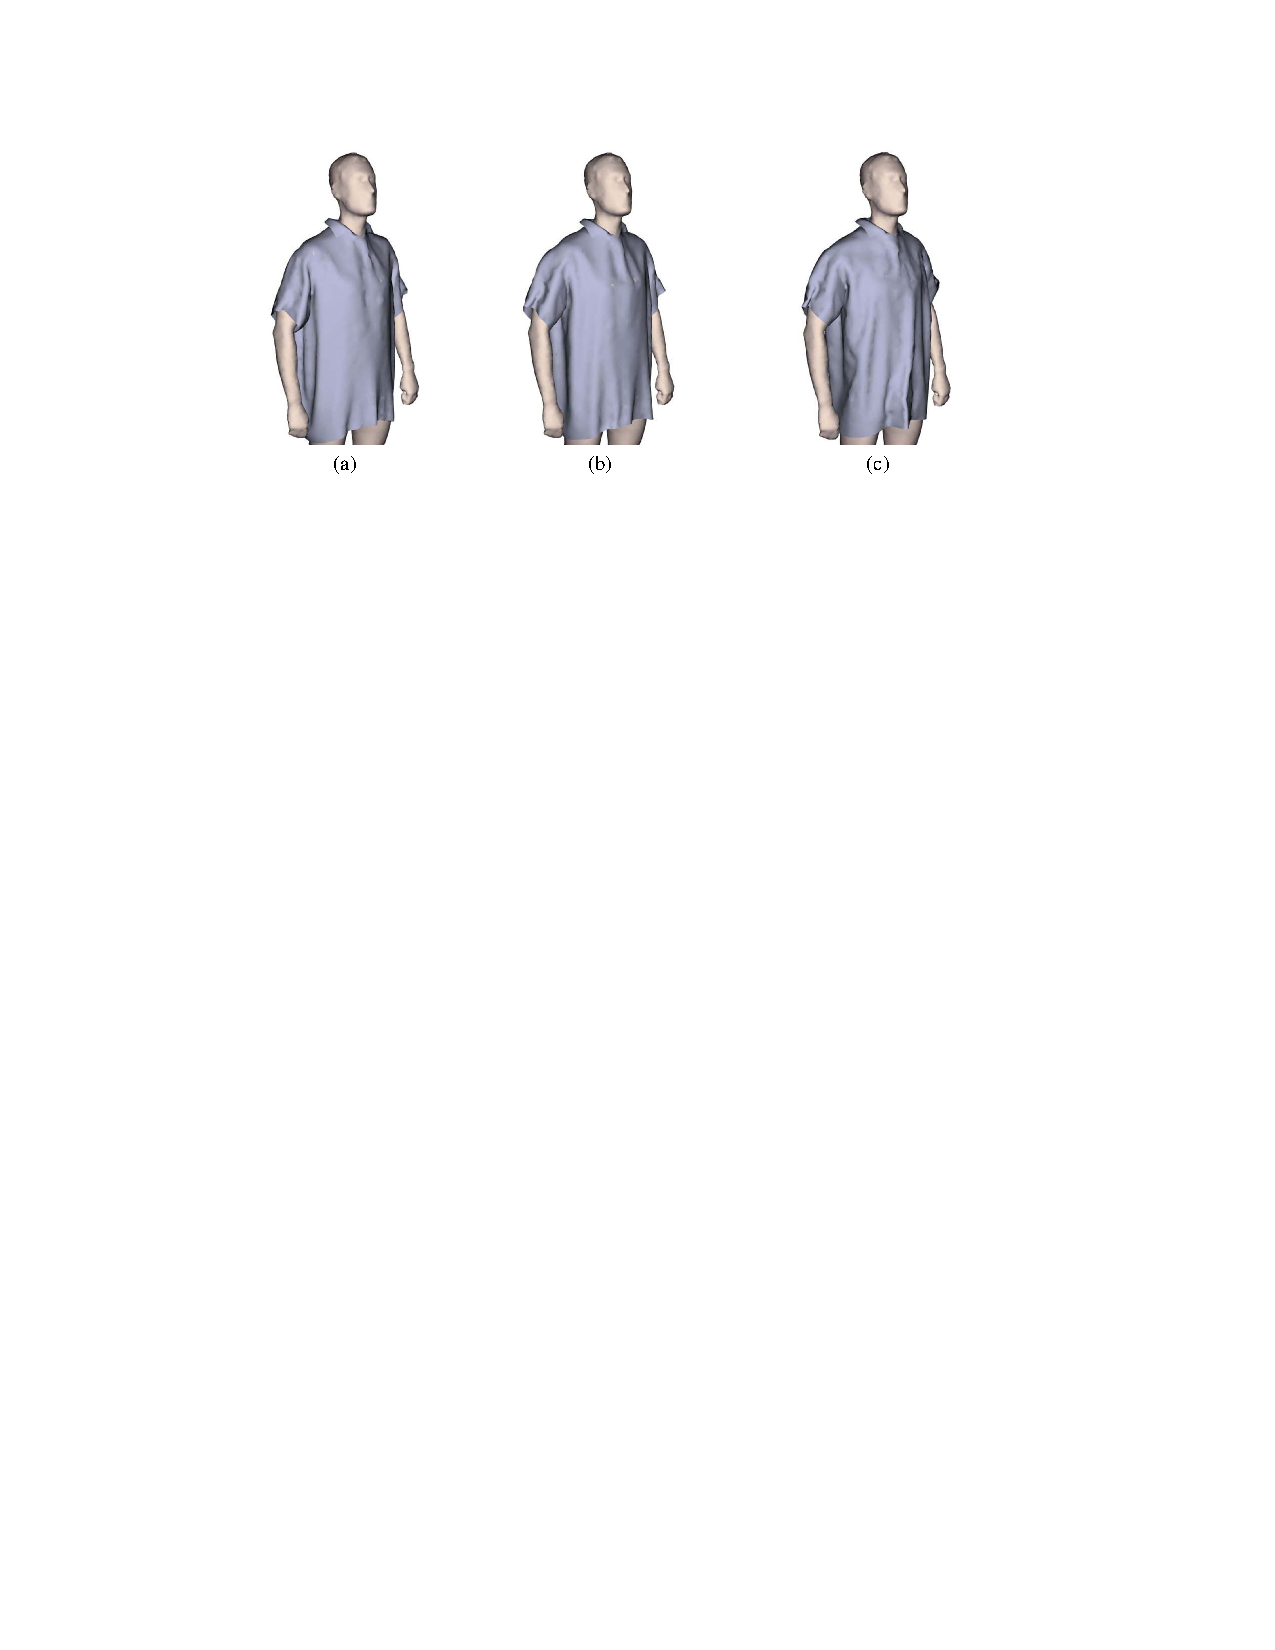
\includegraphics[width=12cm]{chapter7/shirt.pdf}
\caption[A shirt shown with different material properties]{A shirt shown with different material properties: (a) wool/viscose, (b) wool and (c) polyester/polyacrylics/acetate. Image courtesy of \cite{Etzmuss03}.}
\label{chap7:fig-shirt}
\end{center}
\end{figure}

\cite{Thomaszewski06} based their model on the Kirchhoff-Love shell theory and built a subdivision-based finite element formulation similar to \cite{Cirak00}.  They also employed a co-rotational framework to simulate wrinkles and folds of textiles. Although the rotation field is computed for each vertex, they found that using the rotation obtained for the barycentre of all vertices involved was sufficient. More recently, \cite{Allard09} also used a co-rotational finite element formulation to model the membrane of the lens capsule in a cataract surgery simulator. The goal was to simulate the anisotropic fracture progation during capsulorhexis, the technique used to create a circular opening in the lens capsule. The formulation did not feature bending however. 
%
\begin{figure}[ht]
\centering 
\subfloat[Under gravity]{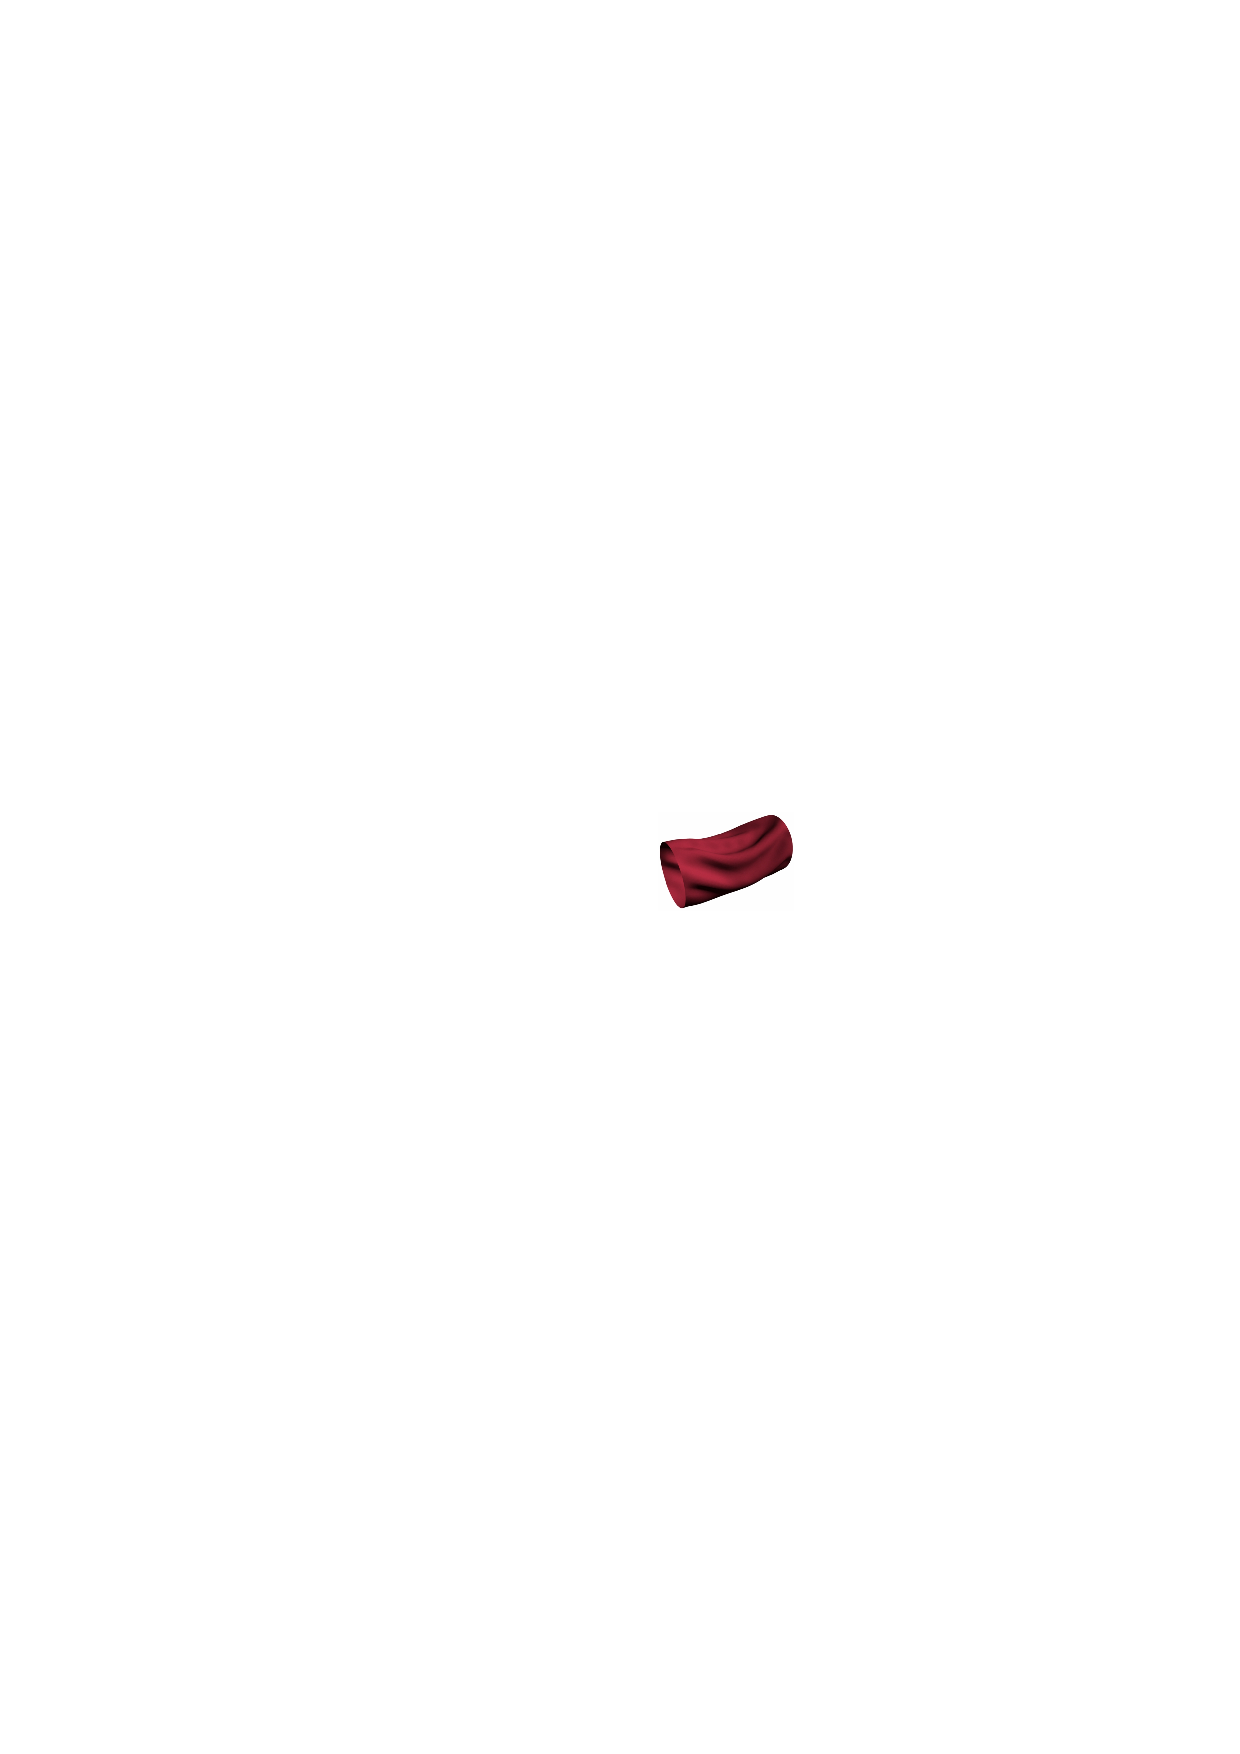
\includegraphics[width=4.5cm]{chapter7/sleeve1.pdf}}
\hfill 
\subfloat[Torsion]{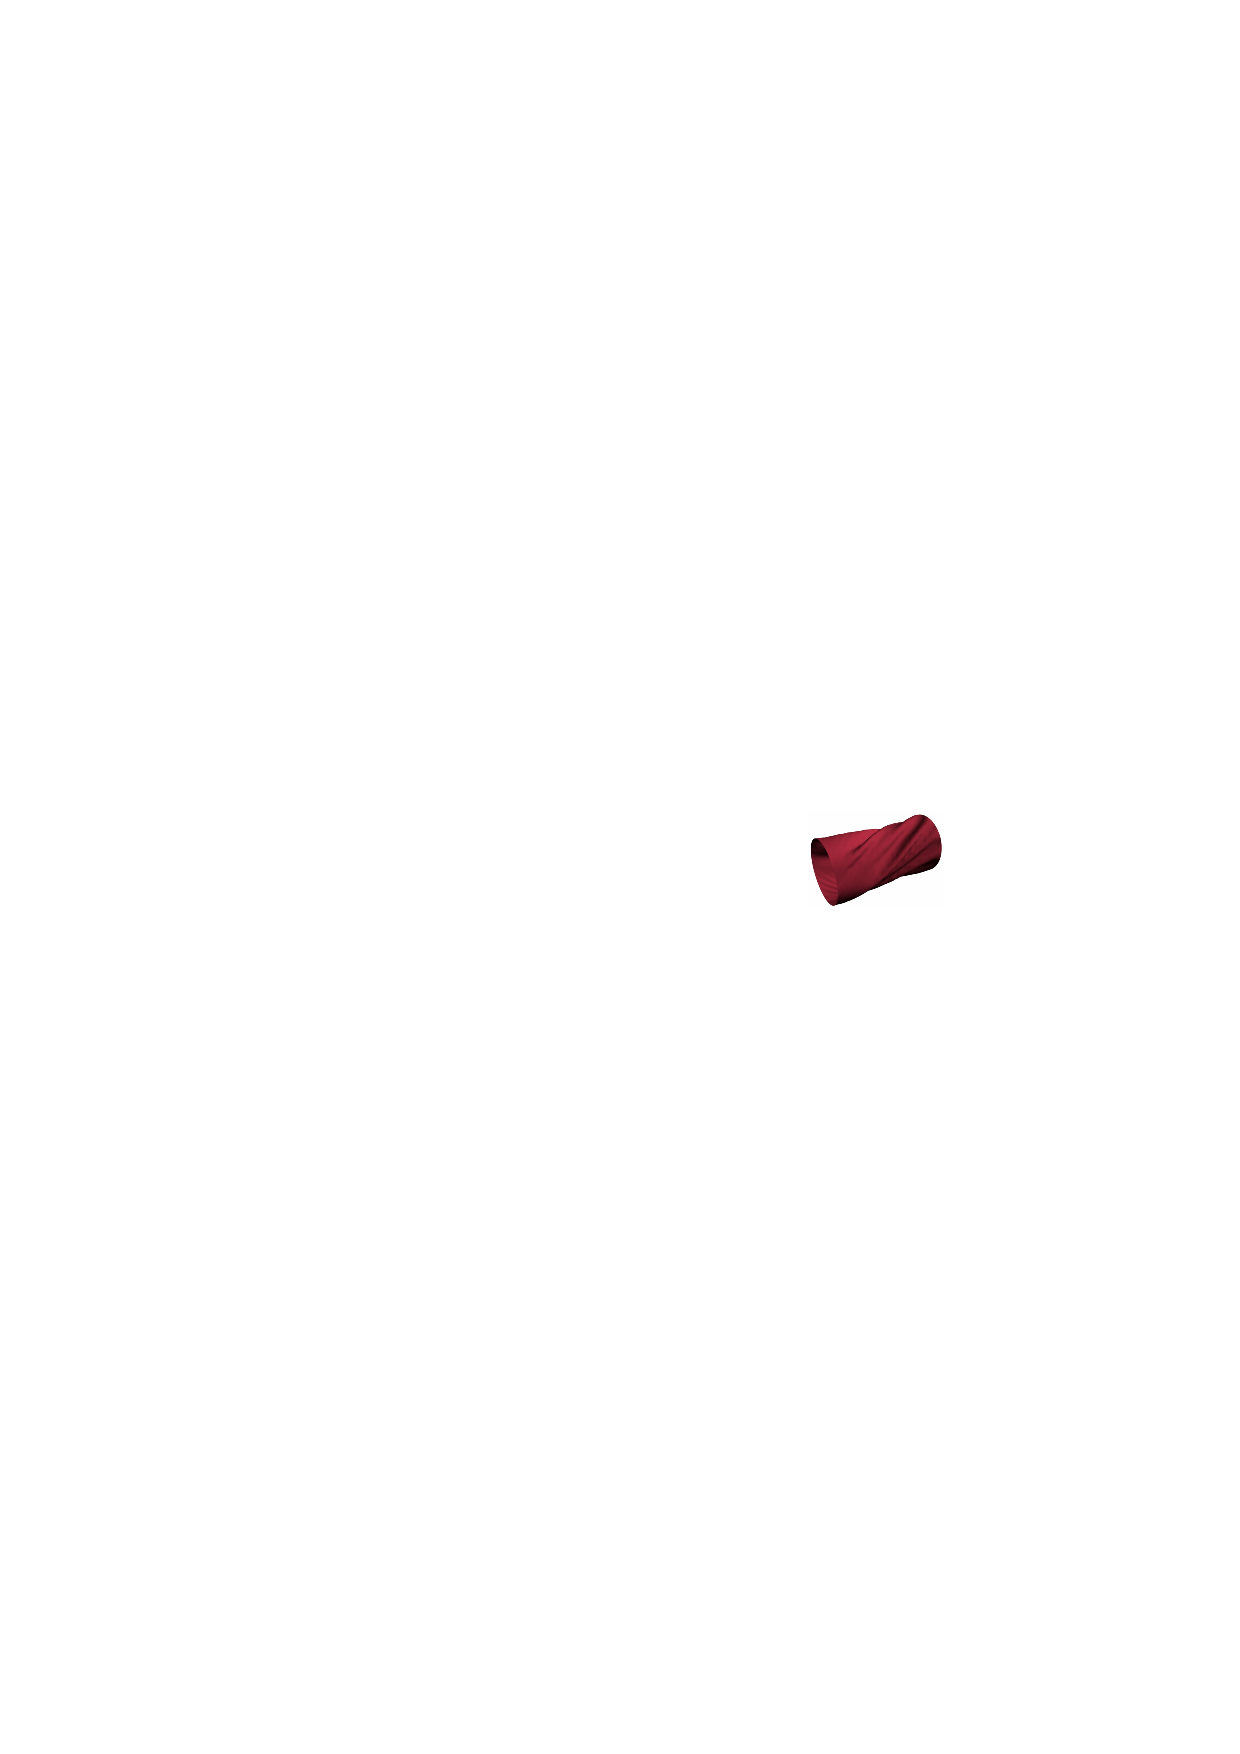
\includegraphics[width=4.5cm]{chapter7/sleeve2.pdf}}
\hfill 
\subfloat[Compression]{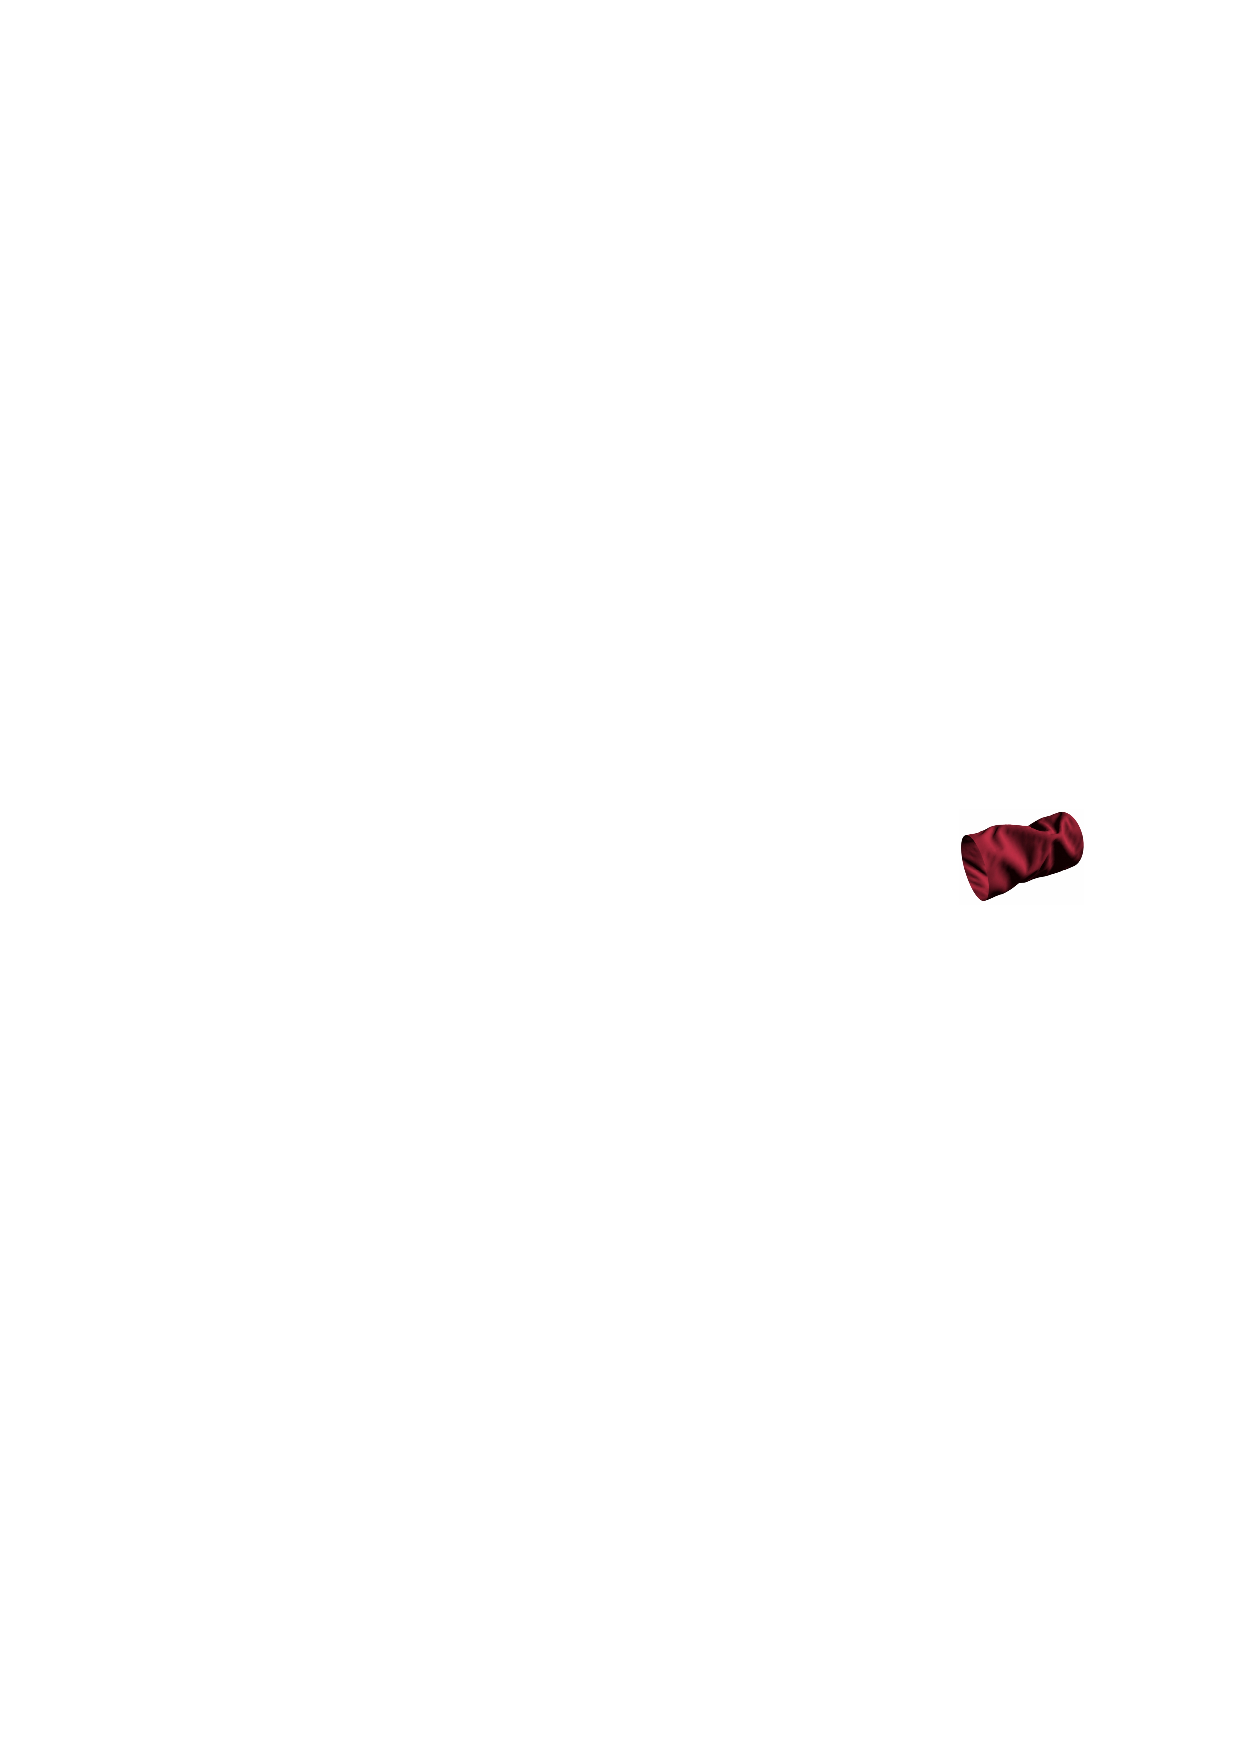
\includegraphics[width=4.5cm]{chapter7/sleeve3.pdf}}
\caption[Different types of folds on a garment's sleeve ]{Different types of folds on a garment's sleeve. Images courtesy of \cite{Thomaszewski06}.}
\label{chap7:fig-sheet}
\end{figure}

Regarding medical applications, some attempts have been made to apply complex shell finite element model to simulate anatomical structures. For instance, \cite{Lim05} used an asymmetrical shell element model to simulate the deformation of the mitral valve. The computation of the finite element model was carried out with the commercial software ANSYS. \cite{Conti10} modelled the non-linear and anisotropic mechanical response of the aortic leaflets during the entire cardiac cycle using a shell finite element model in Abaqus FEA. However, these models are not designed for interactive simulation and may need up to dozens of hours to be computed. 


\section{Objectives}

We seek to propose a solution for simulating, in real-time, the deformation of thin anatomical structures. Since \cite{Black91} showed that formulations with only membrane energy were likely to produce significant errors in the stress distribution, this model is required to feature bending. Ideally, this solution would be versatile and allow us to simulate thin objects with various shapes and material properties with good accuracy. In this regard, methods derived from continuum mechanics are the most appropriate. In some situations, a thin plate model would not correctly capture the deformation of some objects and therefore a shell formulation was retained for more flexibility. To the best of our knowledge, no real-time shell finite element method was presented in the field of medical simulation. \TODO{need to triple-check this...} 

In the next section, we will first introduce our co-rotational triangular shell finite element model and show how to efficiently apply this model to simulate the implant deployment in cataract surgery. In a second time, we will present a technique to mesh complex anatomical shapes with curved triangles, hence allowing us to model, in real-time, any anatomical structures with our co-rotational shell FEM in an optimal way. 

% The key idea is to model the physical shell as a surface but endowed with mechanical properties in the form of elastic resistance to stretching and bending forces. 


